\documentclass[usenames,dvipsnames]{beamer} 

\usepackage[orientation=portrait,scale=1.5,size=a1]{beamerposter} 
\usepackage{svg}
\usepackage{tcolorbox}
\usepackage{background}
\usepackage{lipsum}  
   
\usebackgroundtemplate{\includesvg[height=\paperheight]{template}}%
\setbeamercolor{title}{fg=white} 
\setbeamercolor{author}{fg=white} 
\setbeamercolor{institute}{fg=white} 
\setbeamercolor{date}{fg=red}  
 
 % Poster title
\title{\Huge \textbf{The NeXus Constructor}} 
\subtitle{\Large Visualising the Configurations of Neutron Experiments with Qt for Python}
\author{\large Jack Harper\inst{1}, Dolica Akello-Egwel\inst{1}, Matthew Jones\inst{1,}\inst{2}, Dominic Oram\inst{1}, Jonas Nilsson\inst{3}, Tobias Richter\inst{3} }
\institute{\normalsize   
\inst{1} ISIS Facility, Rutherford Appleton Laboratory, Didcot, Oxfordshire, UK  \,\, 
\inst{2} Tessella Ltd., Abingdon, Oxfordshire, UK
\inst{3} European Spallation Source, Lund, Sweden
}
% Remove Date
\date{}

% Remove Beamer Navigation Symbols
\setbeamercolor*{frametitle}{bg=}
\setbeamertemplate{navigation symbols}{}

\begin{document}
\begin{frame}[t]
  
\maketitle

\begin{columns}[t]  
\begin{column}{0.47\paperwidth}

%%%%%%%%%%% Start of Column 1 %%%%%%%%%%
\begin{tcolorbox}[colback=white,colframe=white,title=Introduction,coltitle=blue]
Neutron experiments would be pointless without data analysis and visualisation. In order to perform accurate data analysis, you need to lay out where each component is with high precision, such as neutron detectors, which capture the pulse of energy after going through a sample, or disk choppers, which cut the beam of neutrons up. 
\end{tcolorbox}

\bigskip

\begin{tcolorbox}[colback=white,colframe=white,title=Neutron Facilities and the NeXus Standard,coltitle=blue]
\lipsum[1-3]
\end{tcolorbox}

\bigskip

\begin{tcolorbox}[colback=white,colframe=white,title=The NeXus Constructor,coltitle=blue]
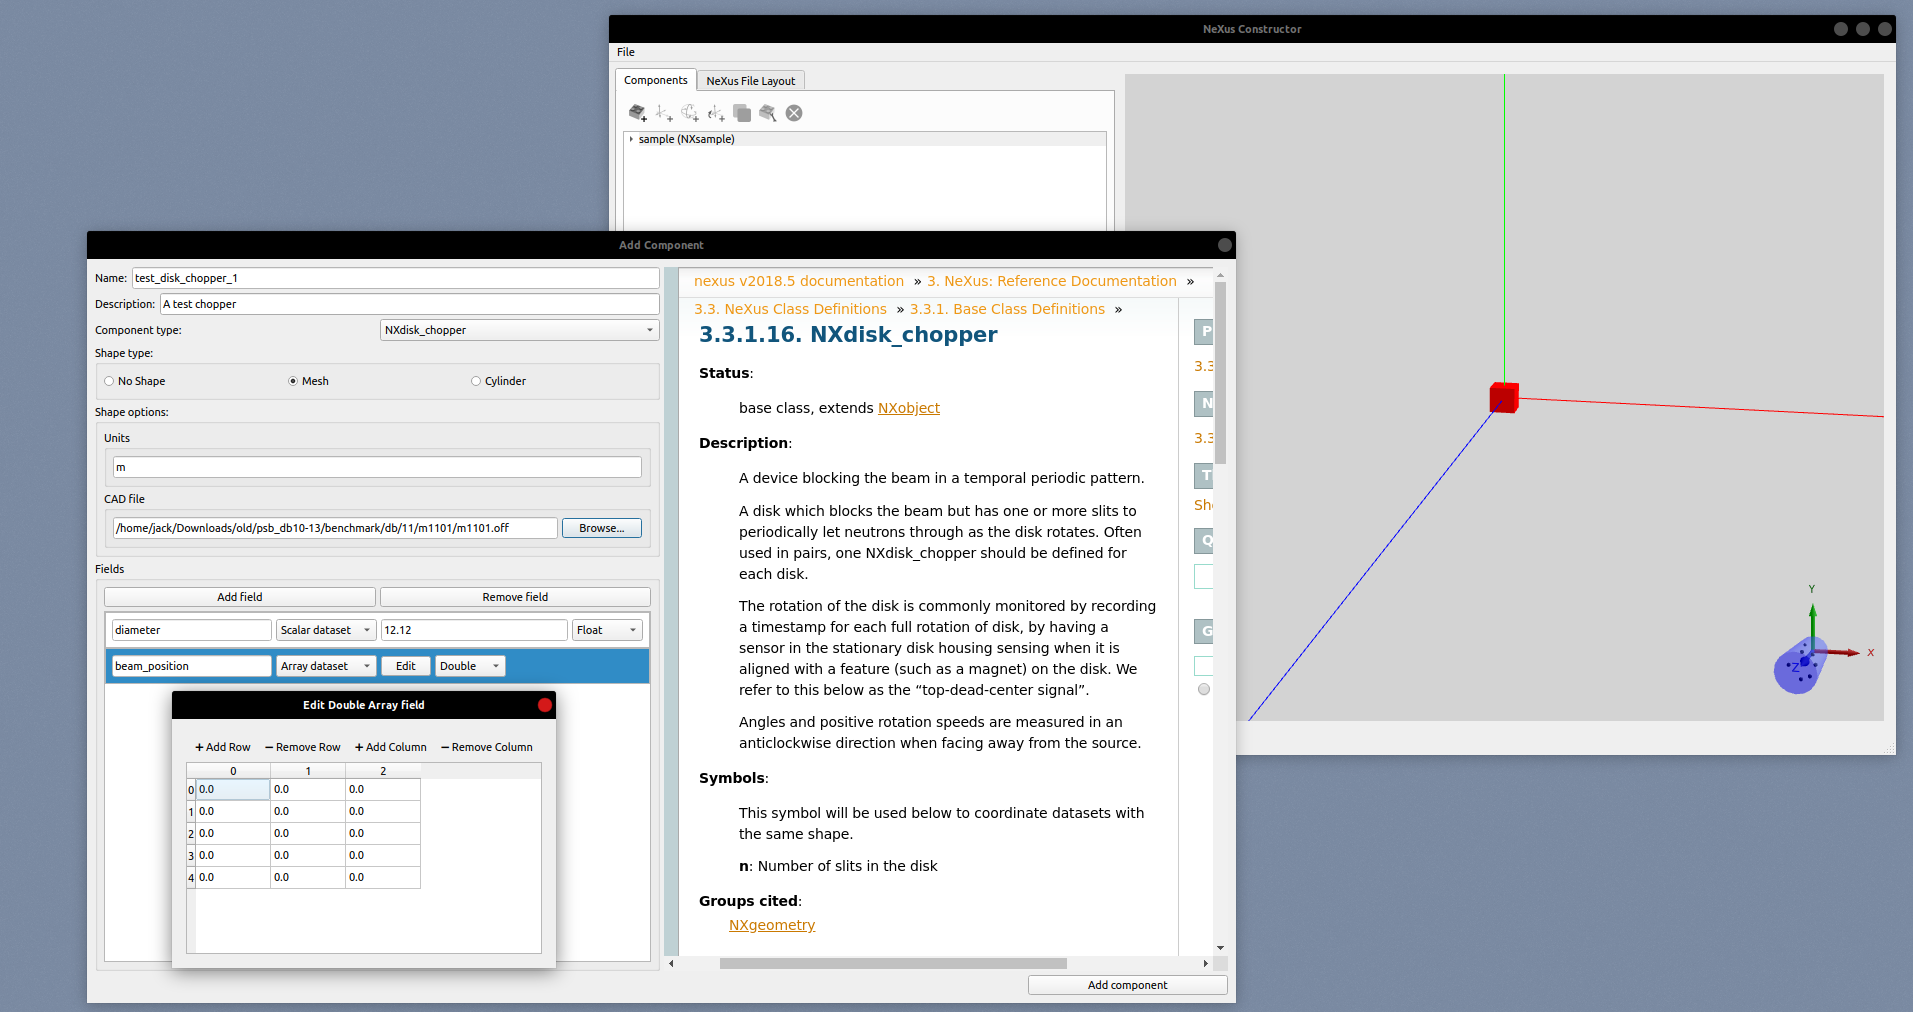
\includegraphics[width=\linewidth]{screenshot.png}
\lipsum[2]
\end{tcolorbox}

\end{column}   
%%%%%%%%%% End of Column 1 %%%%%%%%%%

%%%%%%%%%% Start of Column 2 %%%%%%%%%%
\begin{column}{0.47\paperwidth}  

\begin{tcolorbox}[colback=white,colframe=white,title=Qt for Python,coltitle=blue]
We are using Qt for Python(PySide2) for the NeXus Constructor's graphical user interface. These are the official bindings for Qt 5 C++ API, provided by the Qt company. 

We are taking the Qt-Widgets approach to developing the NeXus constructor, as the tooling for Qt-Quick/QML seems to be a bit lacking and some of the bindings are not pythonic, and rather use C++-like idioms. 

Since version 5.12 PySide2 has included the Qt3D module in Qt5. We are utilising this with our 3d View of components in the neutron experiments. Qt3D provides a high-level interface to OpenGL which allows us to display the geometry information of components as well as an animated pulsed neutron beam.

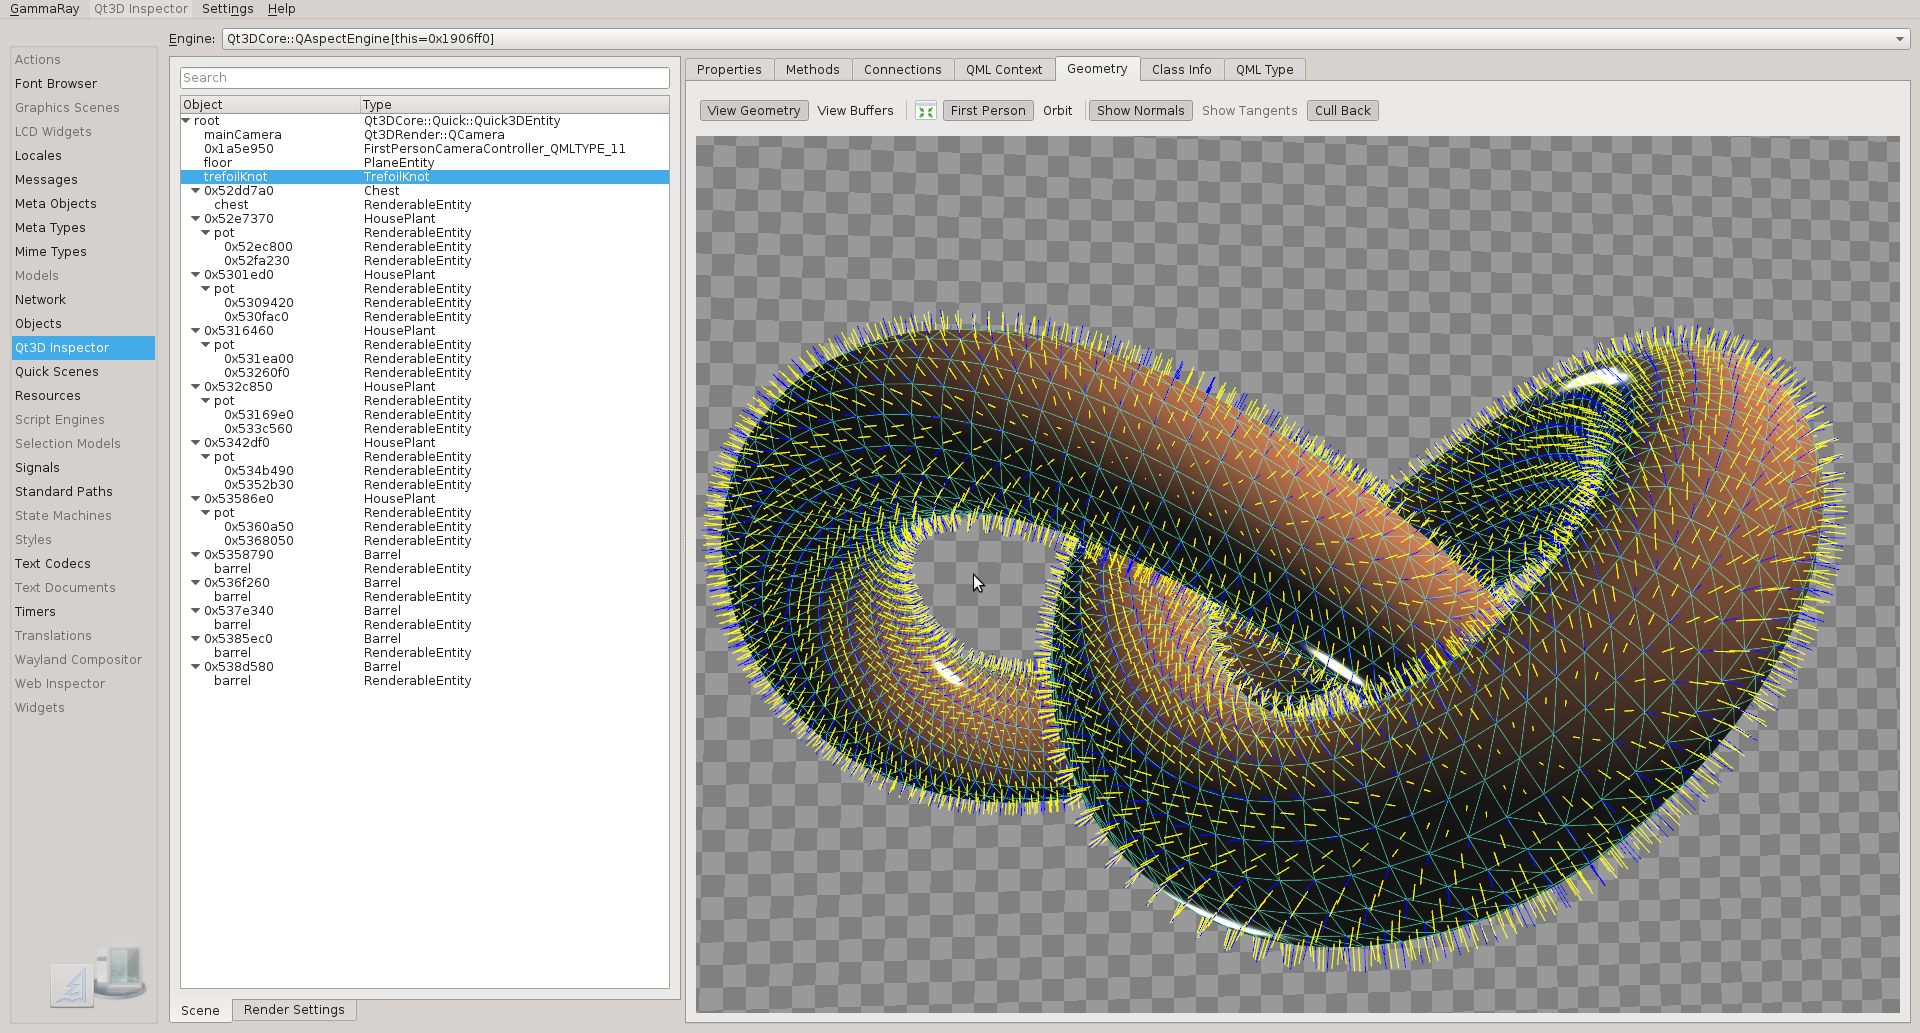
\includegraphics[width=\linewidth]{qt3d.png}

\end{tcolorbox}

\bigskip


\bigskip

\begin{tcolorbox}[colback=white,colframe=white,title=Conclusion,coltitle=blue]
\lipsum[2]
\end{tcolorbox}

\end{column}
%%%%%%%%%% End of Column 2 %%%%%%%%%%  
\end{columns}
 
\end{frame}
\end{document}
 